\documentclass[10pt,twocolumn]{article}

\topmargin -0.5in
\oddsidemargin 0.0in
\textwidth 6.5in
\textheight 9in

\usepackage{graphicx}
\usepackage{amsfonts}
\usepackage{amsmath}
\usepackage{hyperref}

\begin{document}

%Title of paper
\title{Using Network Structure to Learn Category Classification in Wikipedia}

\author{Caitlin Colgrove, Julia Neidert, Rowan Chakoumakos}

\date{\today}

\maketitle

\section{Introduction}

Wikipedia, founded in 2001, is a massive, collaboratively-edited online encyclopedia. As of November 2011, the site has more than 20 million articles available in 282 different languages. The site is maintained by a vibrant community of editors, who supervise the editing process to ensure quality and consistency. 

The body of a Wikipedia article consists primarily of text, images, and hyperlinks to other articles. In addition to article content, each page is also placed into various relevant categories of articles. The editors of Wikipedia maintain this category hierarchy, manually labeling articles with the most appropriate categories. These categories are often used as the gold standard for semantic NLP problems, such as finding document topics [9]. Categories can also be useful in navigation of Wikipedia, whether simply finding related articles or attempting to find longer paths through the network.

However, as Wikipedia continues to grow, manually labeling categories becomes more and more difficult. With over 80,000 categories, the monumental task requires its own �Uncategorized Task Force� of Wikipedia editors, whose goal is to categorize uncategorized articles. Even so, many articles remain uncategorized or undercategorized [13].

Fortunately, many articles in Wikipedia have a wealth of information, from the content of the text to the hyperlink network. These features suggest that an automatic classifier of Wikipedia may be a tractable problem. A classifier with reasonable accuracy could greatly lighten the load of the task force, improve the coverage of articles, and possibly identify and correct miscategorized articles. In this paper, we focus on network features to achieve this goal.

\section{Prior Work}

Previous work in categorizing Wikipedia articles has focused on NLP to automatically classify categories [4]. In the paper ``Automatic content-based categorization of Wikipedia articles," Zeno Gatner and Lars Schmidt-Thieme were able to achieve a F-measure on predicting categories between 0.55 and 0.8 using NLP features. Assigning categories, however, does not have to be only based on NLP, but instead can incorporate features derived from the structure and properties of the underlying network.  Qing Lu and Lise Getoor, in their paper ``Link-based Classification," saw a statistically significant increase in performance on Cora, CiteSeer, and WebKB datasets when network features such as the degree distribution were used rather than just content features [7].  

Network based features have also been successfully applied to the Wikipedia network [3, 8].  In ``Predicting Crosslingual Link Prediction," Phillip Sorg and Phillipp Cimian, were able to predict crosslingual links by using mainly network derived features (links that connect concepts across different language versions of Wikipedia) with recall of around 70\% and precision of around 94\% [8]. Therefore, we believe that predicting category links based on only network derived features may result in an increase performance over previous NLP attempts, or at the very least increase in performance when used in combination with NLP.

Other work has been done with the Wikipedia category graph.  In ``Analyzing and Visualizing the Semantic Coverage of Wikipedia and Its Authors," Holloway et al. analyzed the category graph and noted that it contains cycles, is disconnected, and based on the edit history is kept up to date [5].  Holloway et al. created super categories to deal with the unwieldy nature of the Wikipedia category.  Given that many categories may be small, using supercategories for prediction may be more accurate. 

\section{Data}

We are using data from the November 7th, 2011 dump of Wikipedia. Our data includes the mapping from pages to the links on the page (this includes both article links and other types of links like categories) and a mapping from category name to category id. After downloading the initial dumps, we converted the SQL of the dumps into a simple CSV format and imported this into a MongoDB database hosted on Amazon EC2. In order to achieve reasonable database performance to run experiments, we had to use eight EBS drives in RAID 0 formatted with the XFS file system.  MongoDB allows us to store an arbitrary number of calculated features for each Wikipedia page, which enabled us to easily build the network.

\section{Model}

We choose to  treat Wikipedia as a network, with pages as nodes and hyperlinks as edges. Other research [15] has found that the clustering coefficients of the Wikipedia networks are considerably higher than the expected clustering coefficient of a random graph of the same degree distribution. This suggests that the Wikipedia network exhibits community structure. We exploit this property by hypothesising that these communities correspond to categories. We thus use features dependent on the pages close by in the graph, presumably in the same category community, to classify Wikipedia pages.

\subsection{In-links and Out-links}

\subsubsection{Basic Algorithm}

In order to directly take the community structure of the Wikipedia network into account, we consider the count and portion of neighboring pages in a given category. We consider both the number of pages that the page in question contains hyperlinks to (out-links) and the number of pages with hyperlinks to the page in question  (in-links). When classifying a page as a member of a particular category, then, we have four features: 
\begin{itemize}
\item the count of out-links from the page to pages of the category
\item the portion of such pages out of all out-links
\item the count of in-links to the page from pages of the category
\item the portion of such pages out of all in-links
\end{itemize}

We further look at these attributes for different �levels� out from the page in question. A page is in level $n$ of a page if it can be reached by following exactly $n$ links from that page. For a particular page and level $n$ we have four additional features:
\begin{itemize}
\item the count of the paths of length $n$ from the page that lead to pages in the category
\item the portion of such paths out of all possible paths of length $n$ coming from the page
\item the count of the paths of length $n$ to the page that come from pages in the category
\item the portion of such paths out of all possible paths of length $n$ leading to the page
\end{itemize}

This allows us to consider pages further from the page in question that may also be in the category community. In addition, pages that are more connected to the page are given more weight. These features are extracted simply by following out-links and in-links of the graph and maintaining counts of all pages reached and counts of pages reached in a particular category. 

\subsubsection{Heuristic}

Considering levels further and further away from a page becomes more and more computationally expensive. In fact, the increase is exponential, and with on average hundreds of links from each page, this is not a trivial exercise. Thus, in order to compute features for far out levels, we use a heuristic that gives a more equal weighting to all pages of a particular level, reducing the preference for more connected pages.  To do this, we initially find and store all pages of distance 1 away from any page in a particular category (all pages with a hyperlink to a page in the category or linked to from a page in the category). We then use this set of pages to find the counts of linked pages from one level away. That is, we estimate the number of paths to pages in the category at level n by getting the count of all pages linked to by pages in level $n-2$ that are in the set of pages of distance 1 from the category. This does not count duplicate paths from pages in level $n-2$ to pages in level $n$, and also does not disambiguate between in-links and out-links at the last link, but nevertheless provides a useful heuristic for find features involving a wider span of pages. 

\subsection{HITS}

\subsubsection{Basic Algorithm}

The HITS algorithm was originally developed to model the fact that in a search for information on the Internet, there are two distinct types of valuable pages: authorities, which contain the desired information, and hubs, which are lists of authorities. The quality of hubs and authorities are defined in a mutually recursive manner: a good hub points to a lot of good authorities and a good authority is pointed to by a lot of hubs. In fact, the notion of authorities lines up quite well with what we are trying to detect: good examples of pages in a particular category. Thus, the feature we select from this algorithm is the authority score for a node.

The simplest version of HITS initializes a hub score $h_i = 1$ and an authority score $a_i =1$ for each node $i$. Additionally, the algorithm computes the adjacency matrix $M$, where $M_{ij} = 1$ if there is a directed link from node $i$ to node $j$. The algorithm proceeds as follows:

Repeat until convergence:
\begin{enumerate}
\item Update $h = Ma$
\item Update $a = M^Th$
\item Normalize to $\sum_i a_i = 1$, $\sum_i h_i = 1$
\end{enumerate}

HITS is a good model for Wikipedia because of frequent hub pages (for example, any �List of...� article). Additionally, HITS captures weighting of edges in a way that simple counting does not. For example, a page for a movie might be a good hub for the �Actors� category, so a link from this movie to a page has a lot of weight, even though the movie is not even in the category being examined.

\subsubsection{Modification}

As presented above, HITS has a few drawbacks. The principal problem is that if the initial graph is chosen to be all of Wikipedia, the algorithm will output the hubs and authorities for all of Wikipedia, not for a topic specific subset. Additionally, because Markov models converge to a single fixed point regardless of their origin, there is no way to initialize the matrix $M$ to avoid this. However, in his discussion of HITS for websearch, Kleinberg proposes a modification to produce a topic-sensitive subgraph [16]. First, he finds the set of documents that match a query. Presumably, the vast majority of good authorities are located within this set. Consequently, it is highly likely that any good hub points to something in this set. Thus, to obtain a topic-specific subgraph, he takes the graph formed by the queried documents and all the documents that have a direct link to or from this set.

Analogously, we create a topic-sensitive subgraph of Wikipedia. To do this, we take all the members of a category (minus the members we will be testing on) and include every page that links to or from one of these pages. This increases the likelihood that pages important to that topic will have many links within the graph, while pages peripheral to the topic will not.

This suggests a naive approach to calculating the HITS scores for a node.

Repeat for all nodes $i$:
\begin{enumerate}
\item Add $i$ and all of its links to the current graph
\item Calculate the HITS scores for the graph
\item Report $h_i$, $a_i$
\item Remove node $i$
\end{enumerate}

However, this produces a second, purely technical, problem. The subgraph of actors plus their direct connections is around 500,000 nodes, taking about 15 minutes per HITS computation. This makes it infeasible to compute these features on more than a few nodes. With datasets up to 1600 entries in size, we could not afford to run such an expensive computation for each node.

To avoid this, we make the following assumption: if HITS has iterated to convergence on a graph, the addition of a single node will not significantly change the already computed HITS scores. Thus, to approximate the HITS authority scores, we calculate HITS once and cache the hub scores. We then calculate an approximate authority score for each node by taking a simple sum over the hub scores of the nodes that link to it.

\subsection{Classification}

We ran several different learning algorithms on our feature sets: Naive Bayes, Logistic Regression, and SVM�s. We also ran parameter selection algorithms to optimize performance of each learning algorithm, as well as feature selection algorithms in order to find the most significant features. 

\begin{figure*}
\begin{center}
\caption{Results of feature selection}
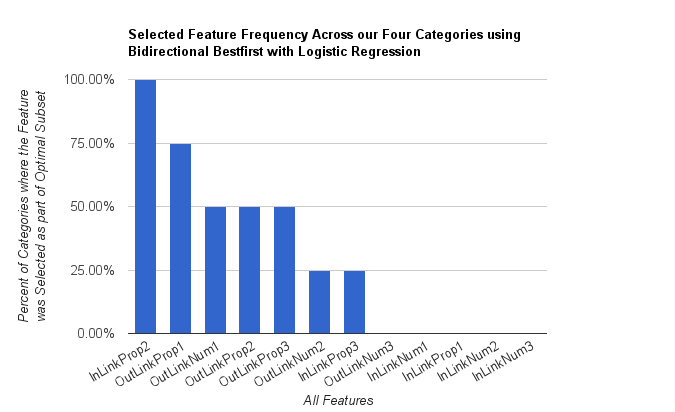
\includegraphics[scale=0.65]{images/selected_features.png}
\end{center}
\end{figure*}

\section{Results}

The goal of our initial classifier was to classify articles as either part of the ``American Actors" category or not. We chose this particular category because it is one of the largest on Wikipedia (almost 25,000 pages), which ensures that there will be many positive examples. We also ran the classifier on the ``American Musical Theater Actors" category, which is a subcategory of the ``American Actors" category , on the ``Desserts" category, and on the ``Graph Theory" category, each of which contains a few thousand pages.

\begin{figure}
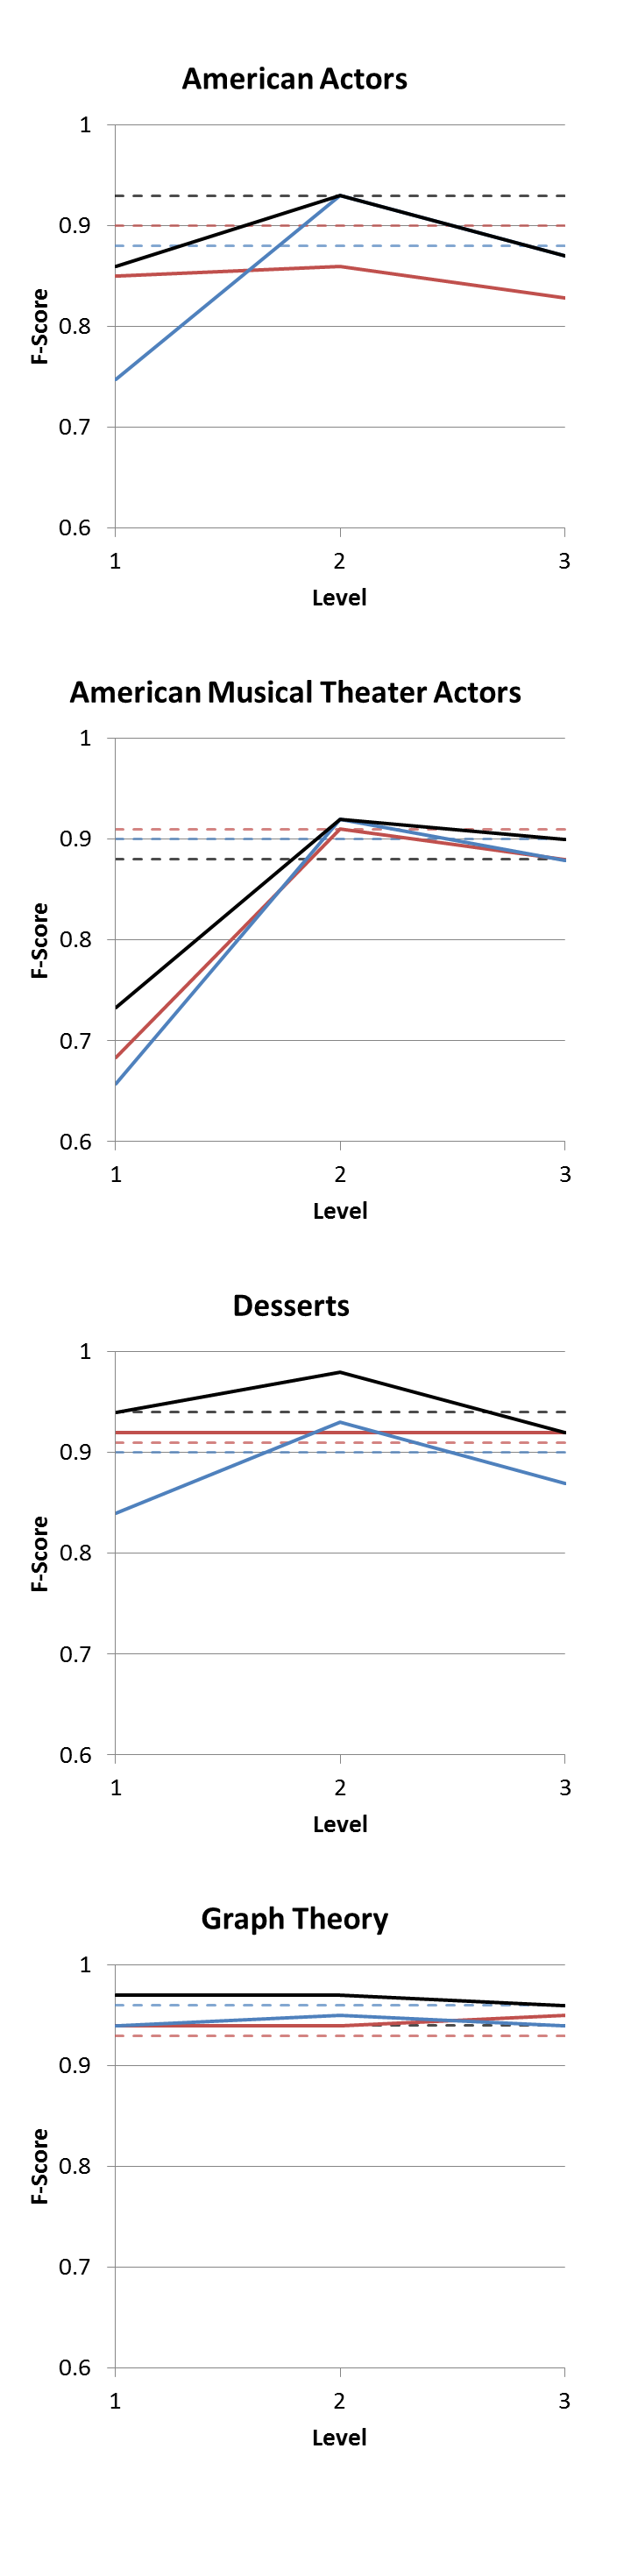
\includegraphics[scale=1]{images/levelInOutPlots.png}
\end{figure}

\begin{figure}
\caption{Performance of classifier at different levels of in and out links on various categories}.
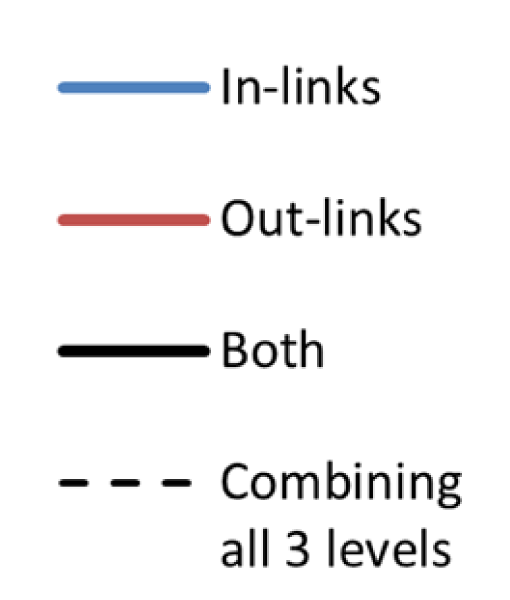
\includegraphics[scale=0.7]{images/levelInOutPlotsLegend.png}
\end{figure}


\subsection{Features}

For the American Actors category, the out-link and in-link features turned out to be best subset of features.  In order to perform features selection, we used the meta classifier WrapperSubsetEval to optimize for the f-score of logistic regression classifier over five folds.  To select which subsets of features that would be tested, we used bi-directional best first search with backtracking up to fifteen steps.  We wanted to test whether the selected features generalized across different categories.  Thus, we performed this feature selection for all four categories (Figure [1]).  InlinkProp2, which is the the proportion of in links at level 2, was in every optimal subset. In second place showing up in three of the four category optimal subsets was the proportion of out links at level 1.  Half of the level three features never occurred in any of the optimal subsets. Based on this analysis, it appears that most of the useful information is gained in the earlier levels, which reduces the computation complexity of calculating these features. 

We ran the classifier on each pair of the out-link and in-link features individually for each of levels 1 through 3, as well as in combination, for a dataset of 100 pages for each category (see Figure [2]).  The level 2 pages were the most effective predictors for all of the categories. This suggests an alternating link structure where intermediate pages between pages of a particular category are complementary pages that perhaps have attributes that are of the category. Consider the case of actors: actor pages are likely to link to non-actor pages, such as movies or awards, that are likely to link to other actor pages. The effect is also perhaps due to the fact that the level 2 pages include more data points than the level 1 pages but are still close enough to the page in question to be relevant. Interestingly, in every case, out-link features performed better than or as good as in-link features for level 1, but worse for level 2.

Using all of the levels as features typically resulted in f-scores between the single level accuracies. Combining the out-links and in-links at that point in some cases even further decreased the f-score. This shows the troubles involved with dumping many features together and speaks for the benefits of the feature selection we performed. 

The experiments discussed above were all performed using regular feature extraction for the link features. We also ran the link feature extraction with the heuristic discussed earlier in order to get a fourth level of features. Combining all 4 of these features performed identically to combining the true 3-level features, suggesting that looking at levels beyond level 2 do not contribute much. Interestingly, looking at only level 2 features found using the heuristic actually gave better f-scores (0.95!) than the standard level 2 features. This suggests that considering all connected pages equally, rather than preferring more connected pages, is more telling of the category of a page. 

All categories were able to be predicted well, especially looking at level 2 features, but some telling differences did appear. The American Musical Theater Actors category, although a very small subset of the American Actors category, still reached an f-score of 0.92. Its performance on level 1 was significantly lower than for the American Actors category, which makes sense since looking at only level 1 will contain far fewer pages in the category, providing insufficient data. The Desserts category classification achieved an f-score of 0.98, and the Graph Theory category classification achieved an f-score of 0.97. These categories are likely much more self-contained than the actors categories, resulting in these better results when looking at community features. Finally, the Graph Theory categorization performed almost equally well for all levels, suggesting that unlike the other categories, its pages and links are homogeneous and all in the same category. Thus, the community features we extracted were effective in classifying each of the categories we considered.

\begin{figure*}
\begin{center}
\caption{Parameter optimization for SVM algorithm.}
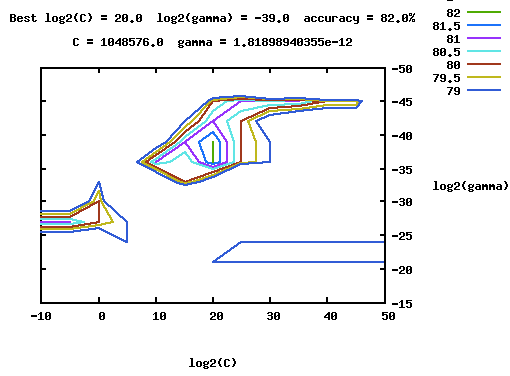
\includegraphics[scale=0.75]{images/svmParameterSelection.png}
\end{center}
\end{figure*}

\begin{figure*}
\begin{center}
\caption{Performance of classifier on different amounts of data.}
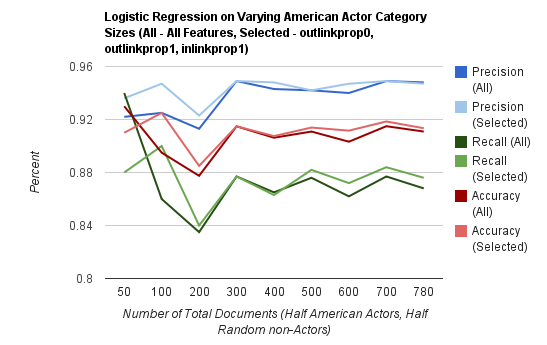
\includegraphics[scale=0.75]{images/varying_datasize.png}
\end{center}
\end{figure*}

\subsection{Algorithms}
	We focused on three learning algorithms for performing the classification based on the features discussed above. Logistic regression performed the best in almost all cases. We also explored Naive Bayes, which was typically a few tenths below logistic regression in f-score. With one exception, SVM algorithms (SMO and LibSVM) had lower f-scores, but had good precision for the American Actors category. Since it is arguably more important to avoid miscategorizing pages than to categorize all the pages, we explored whether we could improve the SVM algorithm accuracy through parameter optimization. By plotting contours of the accuracy values with respect to different $c$ and $\gamma$ values (see Figure [3]), we found that the optimal accuracy for an SVM algorithm would still be significantly lower than for logistic regression. We thus use logistic regression for the remainder of our experiments. 
\subsection{Dataset size}

In order to check whether or not the classifier was over-fitting the rather small dataset of hundred pages (50 American Actor pages and 50 random non-actor pages), we created a dataset of 1560 pages that consisted of 780 American Actor pages and 780 random non-actor pages.  Logistic regression with 10-fold stratified cross validation was able to obtain results of 0.948 precision and 0.868 recall.  Performing this experiment again with feature selection, as described above, resulted in the same 0.947 precision and a slightly higher recall of 0.876.  \footnote{Note our HITS measure appeared to provide redundant information and was not selected as part of the optimal subset. HITS alone had a precision of .917 but had a much lower recall of .412. } We then generated random subsets of increasing size from this dataset to obtain the learning curve for all of the features and the selected features (Figure [4]).  Note that the dip seen at size 400 occurred due to the fact that each size set was a randomly created subset of the larger dataset.  These learning curves confirm that the classification is generalizing and not just over-fitting to the small dataset.

\section{Discussion}

When trying to optimize for various measures of success, we decided that the precision of positive categorization was the most important. Intuitively, not categorizing something as an actor that actually is an actor is better than incorrectly categorizing something that is not an actor as one. High precision here will preserve the quality of the labels, which are important to a significant amount of other research. Our classifier successfully meets this goal, with a best precision of 0.948 when running logistic regression on our largest dataset of American Actors using all of our network features. In addition, the recall on this set was 0.868, which means that we are not sacrificing much recall to achieve these scores. Our best American Actors categorization accuracy of 95\% was achieved by running logistic regression on a smaller dataset considering only level 2 features with a normalization heuristic applied. Since our data was equally split, this accuracy is a good measure of our overall success. The network features approach significantly surpassed the NLP approach presented in [4] in every measure of performance. Even our most simplistic classifiers were on par with the greatest success of the NLP-based classifier . 

Some interesting observations also emerge from our results. Initially, we hypothesized that the implicit community structure of Wikipedia roughly corresponds to the official community structure imposed by the category hierarchy. This hypothesis is supported by the fact that, using only the implicit community structure, we were able to successfully predict the official one.

We also noticed that the most predictive link level is level 2, perhaps indicating that pages tend to link to pages of different categories, but that those pages in turn link back to many pages of the original category in a roughly alternating structure.

\section{Future Work}

Our classifier has proven to be very effective at categorizing Wikipedia pages. Even when we tested narrower categories (such as American Musical Actors), the algorithm performed very well. Because the performance is so good, testing other features would not likely produce a significant improvement. 

However, there are a number of further directions to take this research. The first is to adapt this to fit Wikipedia's categoization system a bit more precisely. Typically, in Wikipedia, categories are not listed as part of the supercategory. They are only officially categorized many levels down in the hierarchy and only implicitly part of the supercategory. As such, extending the classifier to take this into account would produce results more in line with Wikipedia�s current categorization policies. 

The next obvious step would be to write a bot to automatically classify articles. This would be a significant undertaking, because the way our classifier is structured it would have to learn a model for each one of the tens of thousands of categories. For each page, it would have to determine which, if any, of the categories apply. Additionally, human editors could provide feedback on the bot�s classifications, allowing us to apply reinforcement learning to improve the accuracy of the classification. Such a project would use our excellent results to enable people to better navigate and understand the wealth of information that is Wikipedia.

\section{References}

\text{[1]} Chang, Chih C. and Lin, Chih J. ``LIBSVM: a library for support vector machines.� 2001. \url{http://www.csie.ntu.edu.tw/\~cjlin/libsvm}.
\\\\
\text{[2]} Fan, Rong-En and Chang, Kai-Wei and Hsieh, Cho-Jui and Wang, Xiang-Rui and Lin, Chih-Jen. ``LIBLINEAR: A Library for Large Linear Classification.� 2008. \url{http://www.jmlr.org/papers/volume9/fan08a/fan08a.pdf}.
\\\\
\text{[3]} Farin, Jacopo; Tass, Riccardo; and Laniad, David. ``Assigning Wikipedia articles to macro-categories�. 2011. \url{http://www.ht2011.org/demos_posters/ht2011_submission_139.pdf}.
\\\\
\text{[4]} Gantner, Zeno and Schmidt-Thie Lars. ``Automatic content-based categorization of Wikipedia articles�. 2009. \url{http://dl.acm.org/citation.cfm?id=1699765.1699770}.
\\\\
\text{[5]} Holloway, Todd and Bozicevic, Miran and Borner, Katy. ``Analyzing and visualizing the semantic coverage of Wikipedia and its authors.� 2007. \url{http://dx.doi.org/10.1002/cplx.20164}.
\\\\
\text{[6]} Holmes, G. and Donkin, A. ``WEKA: a machine learning workbench�. 2002. \url{http://dx.doi.org/10.1109/ANZIIS.1994.396988}.
\\\\
\text{[7]} Lu, Qing and Lise Getoor. ``Link Based Classification.� 2003. \url{https://www.aaai.org/Papers/ICML/2003/ ICML03-066.pdf}.
\\\\
\text{[8]} Mark Hall, Eibe Frank, Geoffrey Holmes, Bernhard Pfahringer, Peter Reutemann, Ian H. Witten (2009); The WEKA Data Mining Software: An Update; SIGKDD Explorations, Volume 11, Issue 1.
\\\\
\text{[9]} Schonhofen, P. ``Identifying Document Topics Using the Wikipedia Category Network," Web Intelligence, 2006. WI 2006. IEEE/WIC/ACM International Conference on , vol., no., pp.456-462, 18-22 Dec. 2006
doi: 10.1109/WI.2006.92
\\\\
\text{[10]} Sorg, Lipp and Cimiano, Philipp. ``Enriching the crosslingual link structure of Wikipedia - A classification-based approach.� 2008. \url{http://www.aifb.uni-karlsruhe.de/WBS/pso/publications/wikiai08languagelinks.pdf}.
\\\\
\text{[11]} Zlatic, V., M. Bozicevic, H. Stefancic, and M. Domazet. ``Wikipedias: Collaborative web-based encyclopedias as complex networks." Physical Reivew. 2006.
\\\\
\text{[12]} Kleinberg, Jon M. ``Authoritative Sources in a Hyperlinked Environment.�  Proc. 9th ACM-SIAM Symposium on Discrete Algorithms, 1998.
\\\\
\text{[13]} \url{http://en.wikipedia.org/wiki/Special:UncategorizedPages}



\end{document}